\documentclass[]{exam}
\usepackage{listings}
\usepackage{hyperref}
\usepackage{amsmath}
\usepackage{siunitx}
\usepackage{xcolor}
\usepackage{graphicx}
\usepackage{subcaption}

\renewcommand{\familydefault}{\sfdefault}

\definecolor{codegreen}{rgb}{0,0.6,0}
\definecolor{codegray}{rgb}{0.5,0.5,0.5}
\definecolor{codepurple}{rgb}{0.58,0,0.82}
\definecolor{backcolour}{rgb}{0.95,0.95,0.92}

\lstdefinestyle{mystyle}{
	backgroundcolor=\color{backcolour},   
	commentstyle=\color{codegreen},
	keywordstyle=\color{magenta},
	numberstyle=\tiny\color{codegray},
	stringstyle=\color{codepurple},
	basicstyle=\footnotesize,
	breakatwhitespace=false,         
	breaklines=true,                 
	captionpos=b,                    
	keepspaces=true,                 
	numbers=left,                    
	numbersep=5pt,                  
	showspaces=false,                
	showstringspaces=false,
	showtabs=false,                  
	tabsize=2
}
\lstset{style=mystyle}

\title{SBSFEM-tools Documentation}
\author{Sara Patterson}

\begin{document}
	\maketitle
	\tableofcontents
	\section{Installation}
		Clone or download \href{https://github.com/sarastokes/sbfsem-tools}{SBFSEM-tools} and add it to your Matlab path:
		\begin{lstlisting}[language=matlab]
addpath(genpath('C:\...\sbsfem-tools'));\end{lstlisting}
		This includes a few open-source toolboxes: the GUI layout toolbox and JSONlab. If you already have JSONlab, make sure 
		\begin{lstlisting}[language=matlab] 
which loadjson \end{lstlisting} 
		returns the one in \verb|sbfsem-tools\lib\jsonlab-1.5\loadjson.m| sbfsem-tools folder, otherwise there might be some glitches.
	\section{Import}
		\subsection{Import a neuron}
			Open a neuron in Tulip and then open the Python command line (on the bottom toolbar). Create a variable \verb|outputFile| to reflect the file location and name. Then paste in the next two lines.
			\begin{lstlisting}[language=python]
outputFile = "C:\...\filename.json"
params = tlp.getDefaultPluginParameters('JSON Export', graph)
success = tlp.exportGraph('JSON Export', graph, outputFile, params)\end{lstlisting}
			Now go to Matlab, make sure the JSON file is on your path (I save them to the \verb|\demo| folder):
			\begin{lstlisting}
cellName = NeuronNodes(loadjson('filename.json'));\end{lstlisting}
			Now you have a Neuron object! Everything you need is in the GUI which can be accessed by:
			\begin{lstlisting}
cellName.openGUI();\end{lstlisting}
			Everything you need is in the GUI so you are good to go! But bear with me and check out the Organization section...
		\subsection{Add connectivity map}
			This is still a work in progress. Right now you can parse the 1st degree of separation from the .json file into a matlab structure. This is only available from the command line:
			\begin{lstlisting}[language=matlab]
cellContacts = parseConnectivity('c207hops.json');\end{lstlisting}
	\section{Reports}
		This is pretty limited... Right now you can generate a list of the location IDs of unknown synapses and off edges (I use this for incomplete branches). Let me know any other reports that would be of use.
	\section{Save}
	After you edit anything in the Cell Info panel, press the [Add to cell info] button.\\
	To save the entire object, go to \verb|File-->Save|. You will need to at least add a cell number to the Cell Info panel. Note: this will close the GUI but you can always reopen it.
	\section{Export}
		\subsection{CSV}
			This would be easy to add but I am not sure the best layout for the data as I don't use Excel much. If you're interested in this, let me know how you'd like the data arranged.
		\subsection{Plots}
			If you want to keep a graph, use \verb|Export --> Figure| to open the active plot in a new figure window. From there, save/print/copy options are in the File and Edit menu bars.
	
	\section{Organization}
	Some of the things I have planned for the future (particularly comparisons between groups of neurons) will need well-organized file names.. So you'll save yourself some trouble by saving things as follows.
	\begin{itemize}
		\item Copy the \verb|\data| folder and contents to somewhere outside the sbsfem-tools folder (so you don't lose data while updating).
		\item All Neuron objects are saved as the letter `c' followed by the cell's number (like  \verb|c101|). This is because Matlab doesn't like variables beginning with numbers.
		\item Save Neuron objects from TemporalMonkey2 and InferiorMonkey into the \verb|\data\temporal| and \verb|\data\inferior| folders, respectively.
		\item There's no reason to save the .json files, you can delete them after you create the Neuron object.
	\end{itemize}
	
	\section{GUI}
		\subsection{CellData and the Cell Info Tab}
		Setting the cell number is important for saving data but the rest of this tab doesn't have much use yet. Ultimately, this information will be important for connectivity analysis and cell queries.
		\subsubsection{Cell Types}
		If I'm missing any cell types or subtypes, let me know! You can add additional types yourself by going to \verb|defaults\CellTypes.m| or \verb|defaults\CellSubtypes.m|.
		\subsection{3D Plot}
		This plot begins with only the soma node visible. Add/remove synapse types from the checkboxes in the Synapse Table. You can also add a skeleton plot (only the nodes, no edges). \\
		Navigate by changing the azimuth and elevation:\\
		\begin{tabular}{c | c}
			Key & function \\
			\hline
			j & azimuth $\longleftarrow$\\
			l & azimuth $\longrightarrow$\\
			\hline
			i & elevation $\uparrow$\\
			k & elevation $\downarrow$\\
			\hline
			o & increment $\uparrow$\\
			u & increment $\downarrow$\\
		\end{tabular}\\
		These keys default to \ang{22.5} increments but you can increase and decrease this with the `u' and `o' keys. To enable the keyboard control, click on the text box that says: 'Click here to use keyboard control'.
		\subsection{Histograms}
		Navigate between a Distance from Soma histogram and a Z-Axis histogram with the tabs. Use the synapse table to change the bin number.
		\begin{figure}[h]
			\begin{subfigure}{0.5\textwidth}
				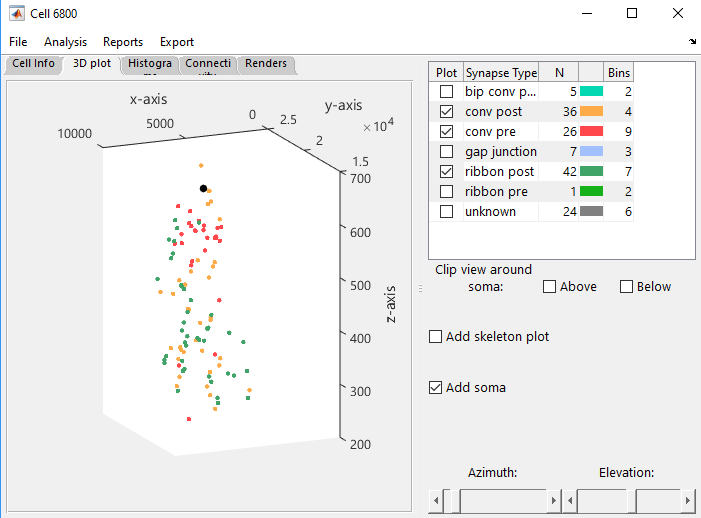
\includegraphics[width=\linewidth]{c6800_plot3}
			\end{subfigure}
			\begin{subfigure}{0.5\textwidth}
				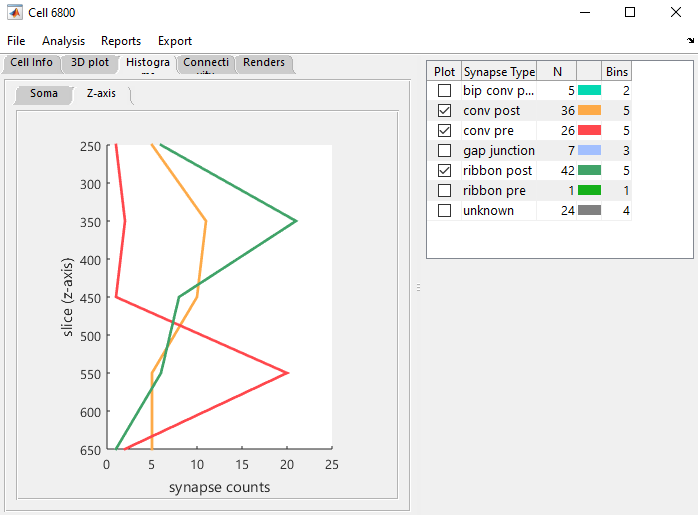
\includegraphics[width=\linewidth]{c6800_histZ}
				\caption{Synapse distribution along the z-axis for a putative AII amacrine cell. The asymmetry in pre- and post-synaptic conventional synapses isn't news but still good to see.}
			\end{subfigure}
		\end{figure}
	\section{Configuration}
		\subsection{Plot Style}
		\begin{enumerate}
			\item \textbf{Synapse colors} - go to \verb|defaults\getStructureColors.m| to change the default colors for each synapse. Matlab accepts RGB values between 0-1. Additionally, I included a function to convert hex to RGB  \verb|hex2rgb('#0000ff')| and a function to convert color names to RGB (\verb|rgb('color name')|) - based on \href{https://xkcd.com/color/rgb/}{XCKD's color survey}. 
			\item \textbf{Markers} - go to \verb|defaults\getMarkersSizes.m|
		\end{enumerate}
		\subsection{Default directories}
		If you get tired of always navigating to your \verb|\data| directories, edit the DefaultSavePath in \verb|\defaults\getFilepaths.m|
\end{document}